\documentclass{shortart}

\usepackage{amsmath, amssymb, amsthm}
\usepackage{plastex}
\usepackage{tikz}

\title{Borwein--Borwein integrals and sums}
\author{Dexter Chua}

\newtheorem{thm}{Theorem}[section]
\newtheorem{lemma}[thm]{Lemma}
\newtheorem{cor}[thm]{Corollary}

\theoremstyle{definition}
\newtheorem{defi}[thm]{Definition}
\newtheorem{eg}[thm]{Example}

\newtheorem*{note}{Note}

\newcommand\Z{\mathbb{Z}}
\newcommand\R{\mathbb{R}}
\DeclareMathOperator\sinc{sinc}
\DeclareMathOperator\sign{sign}
\renewcommand\d{\mathrm{d}}
\begin{document}
The $\sinc$ function is defined by
\[
  \sinc (x) = \frac{\sin (x)}{x}.
\]
A standard contour integral tells us
\[
  \int_{-\infty}^\infty \sinc (x) \;\d x = \pi.
\]
Alternatively, we can observe that
\[
  \sinc (x) = \frac{1}{2} \int_{-1}^1 e^{i k t}\;\d k.
\]
So up to some factors $\sinc x$ is the Fourier transform of the indicator function of $[-1, 1]$. The preceding integral of $\sinc x$ can be thought of as the value of the Fourier transform at $0$. Applying the Fourier inversion formula and carefully keeping track of the coefficients gives us the previous calculation.

David and Jonathan Borwein\footnote{David Borwein being the father of Jonathan Borwein} observed that we also have
\[
  \begin{aligned}
    \int_{-\infty}^\infty \sinc (x) \sinc \left(\frac{x}{3}\right) \;\d x &= \pi,\\
    \int_{-\infty}^\infty \sinc (x) \sinc \left(\frac{x}{3}\right)\sinc \left(\frac{x}{5}\right) \;\d x &= \pi,\\
    \int_{-\infty}^\infty \sinc (x) \sinc \left(\frac{x}{3}\right) \sinc \left(\frac{x}{5}\right) \sinc \left(\frac{x}{7}\right) \;\d x &= \pi.
  \end{aligned}
\]
This pattern holds up until
\[
  \int_{-\infty}^\infty \sinc (x) \sinc \left(\frac{x}{3}\right) \cdots \sinc \left(\frac{x}{13}\right) \;\d x = \pi.
\]
Afterwards, we have
\[
  \int_{-\infty}^\infty \sinc (x) \sinc \left(\frac{x}{3}\right) \cdots \sinc \left(\frac{x}{15}\right) \;\d x = \frac{467807924713440738696537864469}{467807924720320453655260875000} \pi.
\]
As we keep going on, the value continues to decrease.

\section{Direct calculation}
Turns out it is possible to calculate the integrals above by pure brute force, and this gives explicit formulas for the integrals as we see above.

In general, let $a_0, a_1, a_2, \ldots, a_n$ be a sequence of positive real numbers, and consider the integral
\[
  \int_{-\infty}^\infty \prod_{k = 0}^n \sinc (a_k x) \;\d x.
\]

Let us put aside the $\frac{1}{x}$ factors for a moment, and expand out $\prod_{k = 0}^n \sin (a_k x)$:
\[
  \begin{aligned}
    \prod_{k = 0}^n \sin(a_k x) &=  \frac{1}{(2i)^{n + 1}} (e^{i a_0 x} - e^{-i a_0 x}) \prod_{k = 1}^n (e^{i a_k x} - e^{-i a_k x})\\
    &= \frac{1}{(2i)^{n + 1}} \sum_{\gamma \in \{-1, 1\}^n} \varepsilon_\gamma (e^{i b_\gamma x} - (-1)^n e^{-i b_\gamma x}),
  \end{aligned}
\]
where
\[
  b_\gamma = a_0 + \sum_{k = 1}^n \gamma_k a_k,\quad \varepsilon_\gamma = \prod_{k = 1}^n \gamma_k.
\]
Note that each of the terms in the right-hand sum is some sort of trigonometric function, depending on the value of $n$ mod $2$.

The original integral was
\[
  \int_{-\infty}^\infty x^{-n - 1} \prod_{k = 0}^n \sin(a_k x)\;\d x.
\]
Since $\sin(a_k x)$ has a simple zero at $x = 0$, we know from this expression that we can integrate this by parts $n$ times and have vanishing boundary terms:
\[
  \int_{-\infty}^\infty x^{-n - 1} \prod_{k = 0}^n \sin (a_k x)\;\d x = \frac{1}{n!} \int_{-\infty}^\infty \frac{1}{x} \frac{\d^n}{\d x^n} \prod_{k = 0}^n \sin (a_k x)\;\d x.
\]
We now use the expression above to compute this $n$-fold derivative, and get
\[
  \begin{aligned}
    \int_{-\infty}^\infty \prod_{k = 0}^n \frac{\sin(a_k x)}{x} \;\d x &= \frac{1}{n!}\int_{-\infty}^\infty \frac{1}{x} \frac{1}{2^n} \sum_{\gamma \in \{-1, 1\}^n} \varepsilon_\gamma b_\gamma^n \sin (b_\gamma x) \;\d x \\
    &= \frac{\pi}{2^n n!} \sum_{\gamma \in \{-1, 1\}^n} \varepsilon_\gamma b_\gamma^n \sign (b_\gamma).
  \end{aligned}
\]
We claim this is equal to $\frac{\pi}{a_0}$ when $a_0 \geq \sum_{k = 1}^n a_k$, and smaller otherwise. Indeed, this is exactly the condition that all the $b_\gamma$ are positive, so that the sign term disappears. The remaining claim is then that
\[
  \sum_{\gamma \in \{-1, 1\}} \varepsilon_\gamma b_\gamma^n = 2^n n! \prod_{k = 1}^n a_k.
\]
Indeed, this follows by considering the $n$\textsuperscript{th} Taylor coefficient of the equality
\[
  e^{a_0 t} \prod_{k = 1}^n (e^{a_k t} - e^{- a_k t}) = \sum_{\gamma \in \{-1, 1\}^n} \varepsilon_\gamma e^{b_\gamma t},
\]
where on the left we use that $e^{a_k t} - e^{-a_k t} = 2 a_k t$.

\section{Fourier transform perspective}
The preceeding calculation was not very enlightening, but at least it gives precise numbers. There is a more enlightening approach, beginning with our previous observation that $\sinc$ is the Fourier transform of the indicator function of $[-1, 1]$, up to some factors.

To get this going, let us first get our conventions straight. We define our Fourier transforms by
\[
  \mathcal{F}\{f\}(k) = \hat{f}(k) = \int_{-\infty}^\infty f(x) e^{-2\pi ikx}\;\d x
\]
Then for any function $f$, we have
\[
  \int_{-\infty}^\infty f(x) \;\d x = \tilde{f}(0).
\]
Why is this useful? In general, it is difficult to say anything about the integral of products. However, the Fourier transform of a product is the convolution of the Fourier transforms, which is an operation we understand pretty well.

With our convention, we have
\[
  \mathcal{F}\{\sinc a x\}(k) =
  \begin{cases}
    \frac{\pi}{a} & |k| < \frac{a}{2\pi}\\
    0 & \text{otherwise}
  \end{cases} \equiv \chi_{a/\pi} (k).
\]
Here for any $a > 0$, the function $\chi_a (x)$ is given by
\begin{center}
  \begin{tikzpicture}
    \draw [->] (-3, 0) -- (3, 0);
    \draw [->] (0, 0) -- (0, 2.5);

    \draw [dashed, blue] (-1, 0) -- (-1, 1.5);
    \draw [dashed, blue] (1, 0) -- (1, 1.5);
    \draw [blue, thick](-1, 1.5) -- (1, 1.5);
    \draw [blue, thick](-3, 0) -- (-1, 0);
    \draw [blue, thick](3, 0) -- (1, 0);

    \node [below] at (1, 0) {$\frac{a}{2}$};
    \node [below] at (-1, 0) {$-\frac{a}{2}$};

    \node [anchor = north east] at (0, 1.5) {$\frac{1}{a}$};
    \node [fill, circle, inner sep = 0, minimum size = 3] at (0, 1.5) {};
  \end{tikzpicture}
\end{center}
Note that the area under $\chi_a$ is always $1$. Fourier transforms take products to convolutions, and convolving with $\chi_a$ is pretty simple:
\[
  (\chi_a * f)(x) = \frac{1}{a} \int_{x - a/2}^{x + a/2} f(u) \;\d u.
\]
In words, the value of $\chi_a * f$ at $x$ is the average of the values of $f$ in $[x - a/2, x + a/2]$.

With this in mind, we can look at
\[
  \int_{-\infty}^\infty \prod_{k = 0}^n \sinc (a_k x)\;\d x = (\chi_{a_0/\pi} * \chi_{a_1/\pi} * \cdots * \chi_{a_n/\pi})(0).
\]
We start with the function $\chi_{a_0}$, which is depicted above. Convolving with $\chi_{a_1}$ gives a piecewise linear function
\begin{center}
  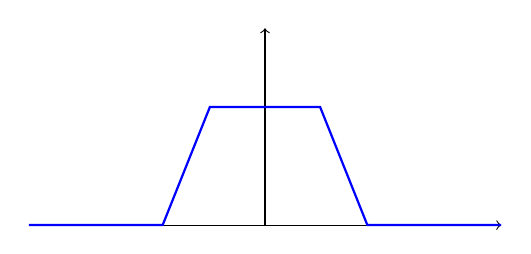
\begin{tikzpicture}
    \draw [->] (-3, 0) -- (3, 0);
    \draw [->] (0, 0) -- (0, 2.5);

    \draw [blue, thick] (-3, 0) -- (-1.3, 0) -- (-0.7, 1.5) -- (0.7, 1.5) -- (1.3, 0) -- (3, 0);
  \end{tikzpicture}
\end{center}
Crucially, when $a_1 \leq a_0$, the value at $0$ is unchanged, since the function is constant on $\frac{1}{\pi}[-a_0, a_0] \supseteq \frac{1}{\pi}[-a_1, a_1]$. The resulting function is constantly $\frac{\pi}{a_0}$ on the interval $\frac{1}{\pi}[-(a_0 - a_1), a_0 - a_1]$.

When we further convolve with $\chi_{a_2/\pi}$, if $a_1 + a_2 \leq a_0$, the resulting function is constantly $\frac{\pi}{a_0}$ on the interval $\frac{1}{\pi}[-(a_0 - a_1 - a_2), a_0 - a_1 - a_2]$. In general, this tells us that as long as $a_0 \geq a_1 + \cdots + a_n$, the integral will still be $\frac{\pi}{a_0}$, and gets smaller afterwards.

\section{Sums}
Let us move on to the series version. We also claim that
\[
  \sum_{n \in \Z} \sinc(n) = \pi.
\]
We also have
\[
  \begin{aligned}
    \sum_{n \in \Z} \sinc(n) \sinc\left(\frac{n}{3}\right) &= \pi\\
    \sum_{n \in \Z} \sinc(n) \sinc\left(\frac{n}{3}\right)\sinc\left(\frac{n}{5}\right) &= \pi.
  \end{aligned}
\]
This continues to hold until $\sinc (\frac{x}{13})$ but fails when we include the $\sinc \left(\frac{x}{15}\right)$ term. Coincidence? We might hope, na\"ively, that the correct result is
\[
  \sum_{n \in \Z} \prod_{k = 0}^N \sinc \left(\frac{n}{2k + 1}\right) = \int_{-\infty}^\infty \prod_{k = 0}^N \sinc\left(\frac{x}{2k + 1}\right) \;\d x.
\]
This is in fact true, for $N\leq 40248$. Number theorists will be delighted to learn that this follows from the Poisson summation formula.

\begin{thm}[Poisson summation formula]
  Let $f: \R \to \R$ be compactly supported, piecewise continuous and continuous at integer points. Then
  \[
    \sum_{n \in \Z} f(n) = \sum_{n \in \Z} \hat{f}(n).
  \]
\end{thm}

The previous observation follows from taking $f(x) = \mathcal{F}\left\{\prod_{k = 0}^N \sinc \left(\frac{x}{2k + 1}\right)\right\}$, which satisfies the hypothesis of the theorem (it is in fact continuous for $n > 0$). The Fourier inversion theorem then tells us $\hat{f}(-x) = \prod_{k = 0}^N \sinc \left(\frac{x}{2k + 1}\right)$. So the right-hand side is the sum in question, and $f(0)$ is the Borwein integral. Our previous analysis shows that the support of $\hat{f}$  is $\frac{1}{2\pi}[-(a_0 + \cdots + a_n), (a_0 + \cdots + a_n)]$. So $\hat{f}$ vanishes at non-negative integers whenever $\sum \frac{1}{2k + 1} < 2\pi$.

\begin{note}
  It is common for the theorem to be stated for Schwarz functions instead. However, our function is not smooth, but the same proof goes through under our hypothesis.
\end{note}

\begin{cor}
  \[
    \sum_{n \in \Z} \prod_{k = 0}^N \sinc a_k n = \int_{-\infty}^\infty \prod_{k = 0}^N \sinc a_k x \;\d x.
  \]
  if $\sum a_k < 2\pi$.
\end{cor}

\begin{proof}[Proof of theorem]
  Set
  \[
    g(x) = \sum_{n \in \Z} f(x + n).
  \]
  Then, $g(0) = \sum_{n \in \Z} f(n)$. Note that the sum converges since $g$ is compactly supported, and is continuous at $0$ since $f$ is continuous at integer points. Of course, it is also piecewise continuous, since in each open neighbourhood, the sum is finite. So we know the Fourier series of $g$ converges at $0$. Recall that the Fourier series is
  \[
    g(x) = \sum_{k \in \Z} \hat{g}_k e^{2\pi i k x},
  \]
  where
  \begin{multline*}
    \hat{g}_k = \int_{\R/\Z} e^{-2\pi i k x} g(x) \;\d x \\
    = \sum_{a \in \Z^n} \int_{[0, 1]} e^{-2\pi i k x} f(x + a)\;\d x = \int_\R e^{-2\pi i k x} f(x) \;\d x = \hat{f}(k).
  \end{multline*}
  So
  \[
    \sum_{n \in \Z} f(n) = g(0) = \sum_{k \in \Z} \hat{g}_k = \sum_{k \in \Z} \hat{f}(k).\qedhere
  \]
\end{proof}
\end{document}
